\documentclass[14pt,a4paper]{article}
\usepackage[utf8]{inputenc}
\usepackage[russianb]{babel}
\usepackage[left=1.5cm,right=1.5cm,top=2cm,bottom=2.5cm]{geometry}
\usepackage{setspace}
\usepackage{indentfirst}
\usepackage{amssymb}
\usepackage{amsmath}
\usepackage{bm}

\usepackage{array}
\usepackage[pdftex]{graphicx}
\usepackage{comment}
\usepackage[table,xcdraw]{xcolor}


\usepackage{verbatim}


\graphicspath{{images/}}
\renewcommand{\baselinestretch}{1.3}

\begin{document}

Для решения нам нужно нарисовать результат работы Черепахи после выполнения алгоритма. Напишем программу, используя библиотеку turtle. Сначала отрисуем фигуры по заданному алгоритму, а затем отметим целочисленные точки, чтобы затем их посчитать. Чтобы картинка не была слишком маленькой, добавим переменную scale, на которую будем умножать все координаты и перемещения.

\begin{verbatim}
from turtle import *

# Ускорение отрисовки
tracer(0)
# Поворот влево, чтобы Черепаха смотрел вдоль оси ординат
left(90)

# Масштаб
scale = 20

# Повтори 2
for _ in range(2):
    # Вперёд 8
    forward(8 * scale)
    # Направо 90
    right(90)
    # Вперёд 18
    forward(18 * scale)
    # Направо 90
    right(90)

# Поднять хвост
up()

# Вперёд 4
forward(4 * scale)
# Направо 90
right(90)
# Вперёд 10
forward(10 * scale)
# Налево 90
left(90)

# Опустить хвост
down()

# Повтори 2
for _ in range(2):
    # Вперёд 17
    forward(17 * scale)
    # Направо 90
    right(90)
    # Вперёд 7
    forward(7 * scale)
    # Направо 90
    right(90)

# Поднимаем хвост, чтобы нарисовать точки
up()
# Рисуем точки с координатами от -30 до 30
for x in range(-30, 30):
    for y in range(-30, 30):
        # Перемещаем Черепаху в точку (x, y)
        goto(x * scale, y * scale)
        # Зелёная точка
        dot(5, "green")


# Отрисовать рисунок
update()
# Конец программы, чтобы рисунок сразу не закрылся
done()
\end{verbatim}

На рисунке увидим следующее:
\begin{center}
    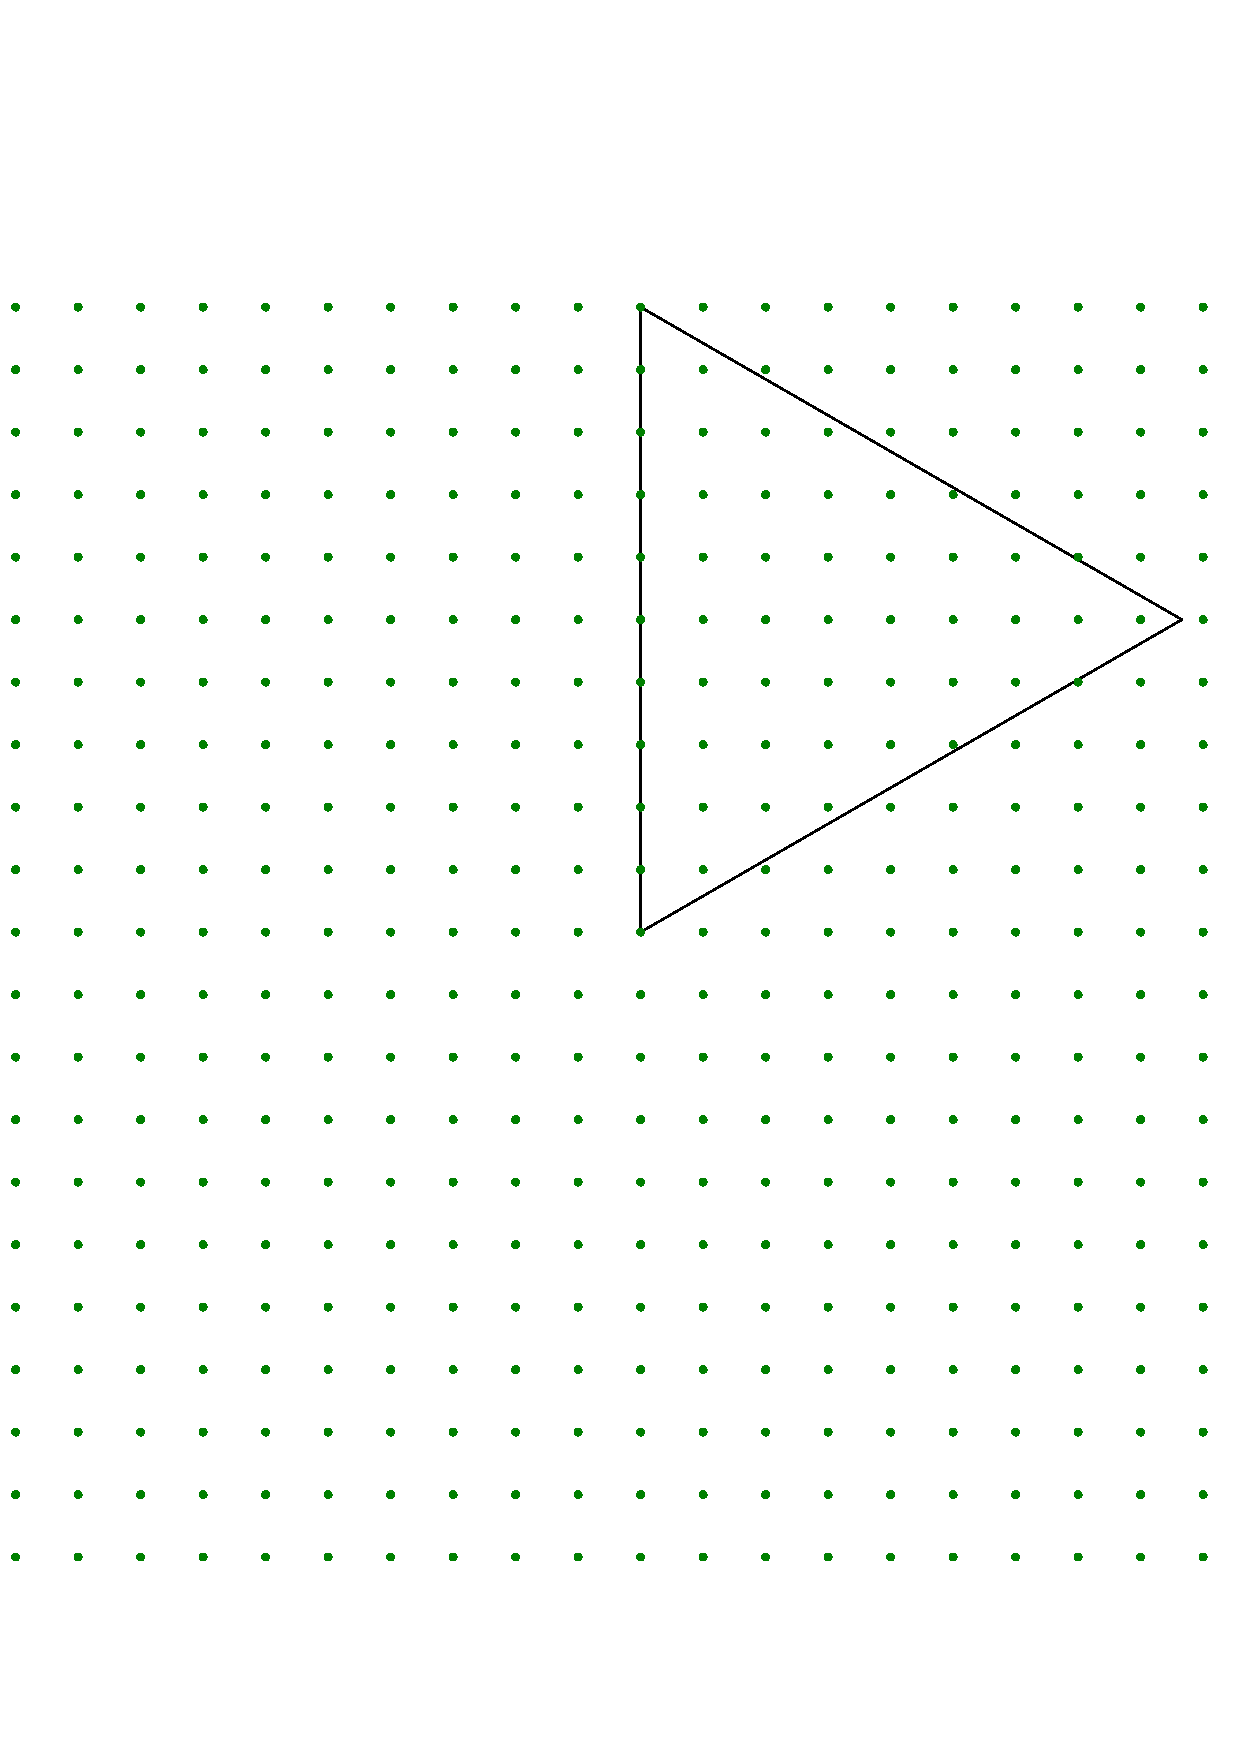
\includegraphics[width=0.4\textwidth]{figure.png}
\end{center}

Посчитаем точки внутри обоих фигур, включая границы, и получим ответ -- 275.

\end{document}
